\setchapterstyle{kao}
% \setchapterpreamble[u]{\margintoc}
\chapter{Research and implementation}
\label{ch:problem}

\begin{figure}[hb]
    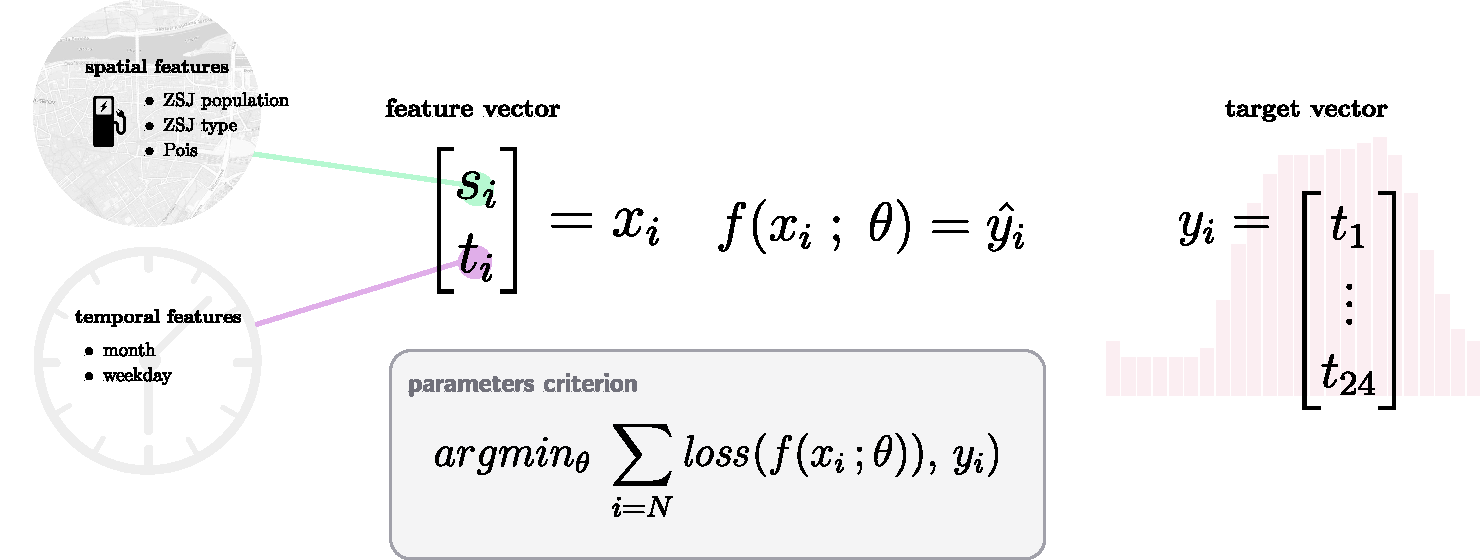
\includegraphics[width=1\textwidth]{diagram-detail}
    \caption[Problem modelling overview]{Problem approach overview}
\end{figure}

In this chapter, the problem will be formulated, and then an approach of solving it will be presented. The choice for the ML model will be discussed as well as its interpretable structure. A way of processing the data, splitting it into training and validation sets will be presented. And then a way to evaluate the model in comparison to other ML models will be described.

\section{Problem statement}

% \begin{marginfigure}
%     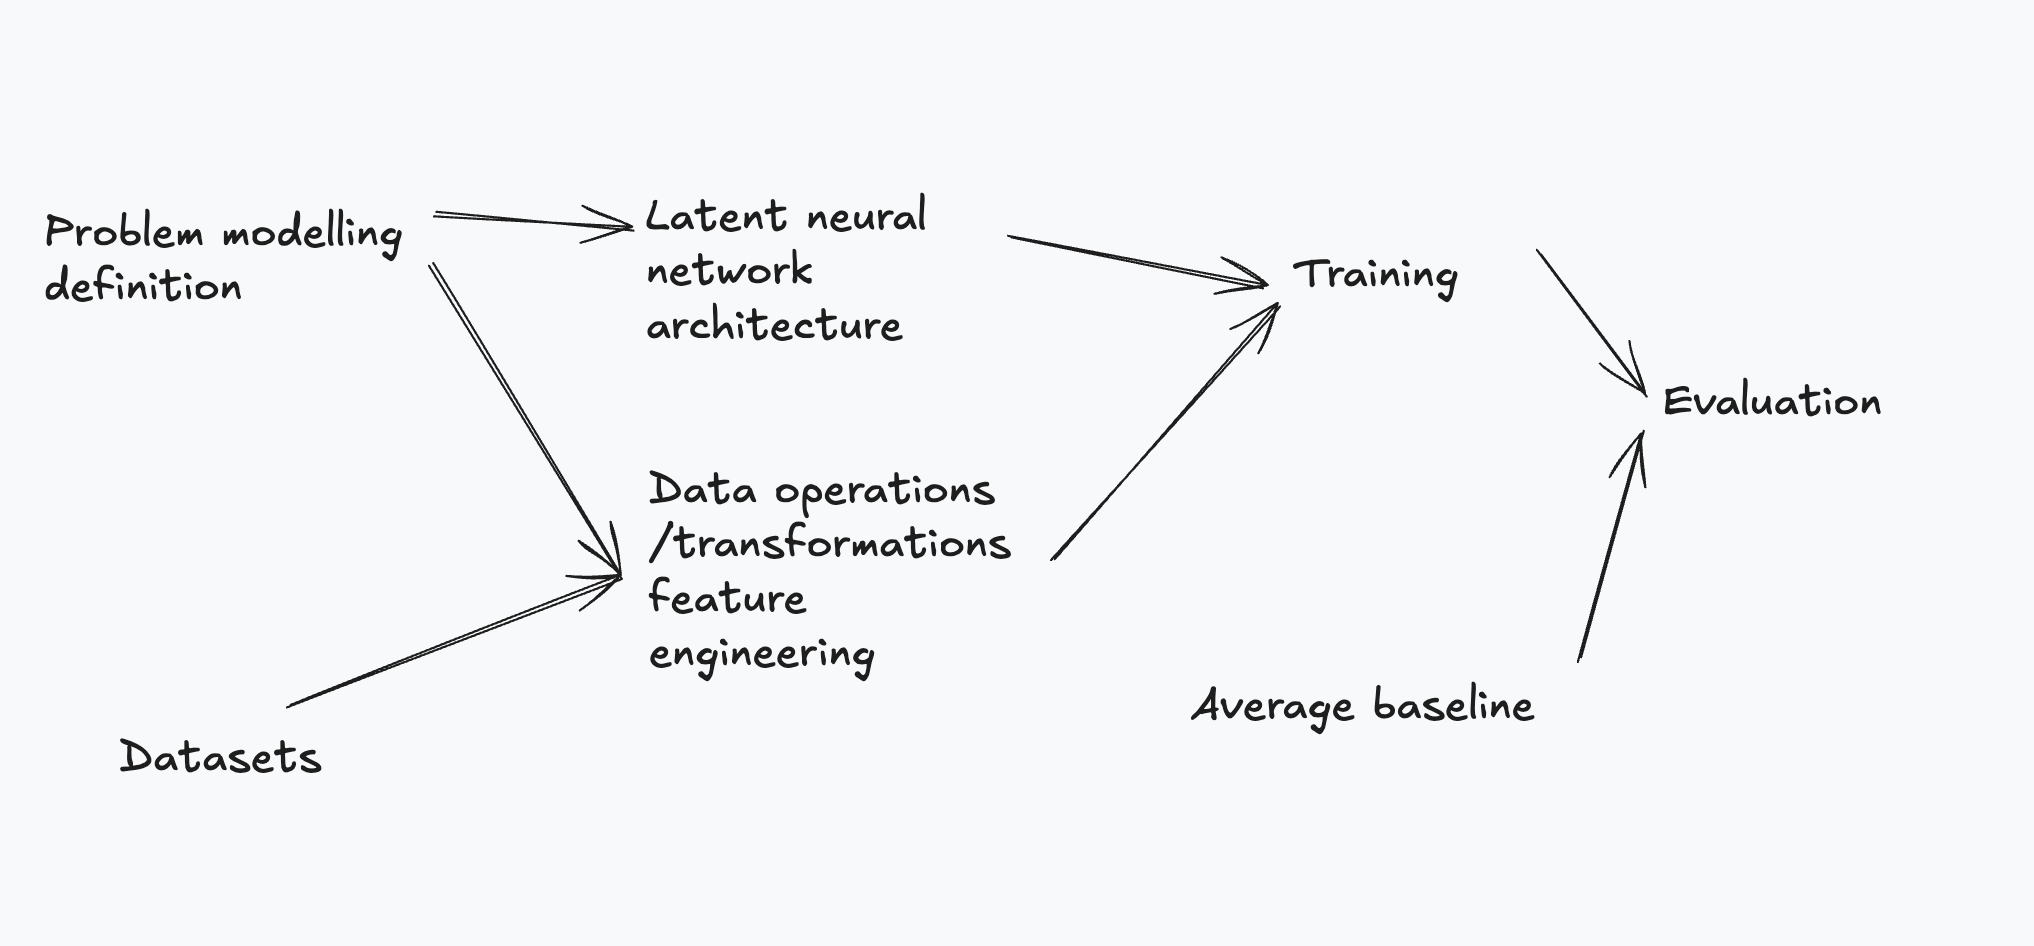
\includegraphics{diagram}
%     \caption[Problem modelling overview]{Chapter content overview.}
% \end{marginfigure}


We will be interested in estimating \acrfull{APC} from some set of features. And will like to know if our data-driven approach is viable.

To formulate how the model will look like, the model $f_\theta$ will execute the following mapping:

\[
    f_{\theta}: X \rightarrow Y
\]

Where $X$ will be the set of all feature vectors and $Y$ will be the set of all targets. The available data are split into \textit{training} \textit{test} and \textit{validation} sets. The first available at training time with goal of the training algorithm to minimize the empirical risk. How those sets are constructed is explained in \ref{sec:dataset-split}


$X \in \mathbb{R}^M$ and $Y\in \mathbb{R}^{24}$. And $| A | = | B | = P$.

The model function $f$ will have trainable parameters $\theta$. And we will be interested in finding such $\theta$ that minimizes the empirical risk:

\begin{equation}
    \mathit{loss_{total}}(f,\theta) = \frac{1}{P} \sum_{(x,y)\in\mathcal{T}} \alpha \cdot a_x + \beta \cdot b_x
\end{equation}

Where:

\begin{equation}
    \begin{split}
        a_x & = \mathit{loss_{power}}
        (\left \lVert f(x_i;\theta) \right \rVert_{1}, \left \lVert y_i \right \rVert_{1}) \\
        b_y & = \mathit{loss_{norm}}
        (\frac{f(x_i;\theta)}{\left \lVert f(x_i;\theta) \right \rVert_{1}}, \frac{y_i}{\left \lVert y_i \right \rVert_{1}})
    \end{split}
\end{equation}


where $\mathit{loss_{power}}$ and $\mathit{loss_{norm}}$ will be individual loss functions. Because we will be interested in model performance in estimating \acrfull{TDPC} and \acrfull{NDPC}. This will match with the chosen NN model architecture that will be discussed further in this chapter.

The use case of the model is to answer the EV charger planners' question: what will be the charger's power consumption if he decides to place a new \acrfull{CS} at a new place in Prague? And he is interested in its behavior given the temporal pattern\sidenote{e.g., how would a new charger at place $x$ perform on Thursdays of February}.

\section{Model features and feature engineering}

The feature vector of the model consist of \textbf{temporal} and \textbf{spatial} parts. Features regarding the charger's capabilities should be present as well, but that will be a limitation of the current chargers dataset that we will work with. The most useful will be the charger's maximum power output. Since that will most certainly influence the charger's average consumption. From this absence, the \acrfull{NDPC} will also be in our interest to estimate. Since the total power consumed might not have that big of an influence on it.

The feature items will fall into two categories divided by the data type. Either they will be categorical or numerical. If they will be categorical, they will be transformed with one-hot encoding. That is, given a category with $n$ items to transform the feature into $n$ binary features, where each binary feature will correspond to one of the possible values. For each observation, exactly one of these binary features will have the value 1, indicating the presence of that categorical value, while all others will be 0.

\marginnote{For example, if we have a categorical feature "day of week" with 7 possible values (Monday through Sunday), one-hot encoding transforms this into 7 binary features: "is\_Monday", "is\_Tuesday", etc. If an observation occurs on Wednesday, then the "is\_Wednesday" feature would be 1, while all other day features would be 0. This transformation allows the model to properly handle categorical variables without imposing an arbitrary ordinal relationship between category values.}

In our case, categorical features like the day of the week, month, and location characteristics will be one-hot encoded before being fed into the model. This will ensure that the model can effectively learn from these categorical variables without the constraints of numerical ordering.

Numerical features, on the other hand, will be standardized by subtracting the mean and dividing by the standard deviation to ensure all features will be on a comparable scale. This normalization process will prevent features with larger scales from dominating the learning process and will help achieve faster convergence during model training.

The feature vector will be constructed in the following way:

\begin{equation}
    \renewcommand*{\arraystretch}{1.5}
    x_i = \begin{bmatrix}
        s_i^T \\
        t_i^T
    \end{bmatrix}
\end{equation}

\textbf{spatial features} $s_i$ will be a vector of spatial features which contents will be described in \ref{tab:spatial-features-table} together with how this feature will be encoded.

\begin{equation}
    s_i = \begin{bmatrix}
        s_i^1  \\
        \vdots \\
        s_i^R
    \end{bmatrix}
\end{equation}

\begin{table*}[h!]
    \def\arraystretch{1.5}
    \caption{Overview of spatial features used in the feature vector.}
    \label{tab:spatial-features-table}
    \begin{tabular}{p{1cm} p{3.5cm} p{1.8cm} p{3.5cm} p{4.5cm}}
        \toprule
        \textbf{Index} & \textbf{Name}                                                       & \textbf{Type} & \textbf{Value from}                  & \textbf{Additional processing}                                                                                             \\
        \midrule
        $s_{1}$        & ZSJ population                                                      & numeric       & charger in ZSJ polygon               & normalization by the polygon area                                                                                          \\
        $s_{2:10}$     & ZSJ type                                                            & categorical   & charger in ZSJ polygon               & one-hot encoding                                                                                                           \\
        $s_{11}$       & ZSJ number of addresses                                             & numeric       & charger in ZSJ polygon               & normalization by the polygon area                                                                                          \\
        $s_{12}$       & Number of people commuting into the district from inside Prague     & numeric       & charger in the district polygon      & normalization by the polygon area                                                                                          \\
        $s_{13}$       & Number of people commuting into the district from outside of Prague & numeric       & charger in the district polygon      & normalization by the polygon area                                                                                          \\
        $s_{14:162}$   & Points of Interest                                                  & numeric       & number of PoIs by euclidean distance & importance calculation (value of single PoI is 1 if its distance from charger is 0, 0 if it is of distance 2km or further) \\
        \bottomrule
    \end{tabular}
\end{table*}

\textbf{temporal features} $t_i$ will be a vector of temporal features which contents will be described in \ref{tab:temporal-features-table} together with how this feature will be encoded.

\begin{equation}
    t_i = \begin{bmatrix}
        t_i^1  \\
        \vdots \\
        t_i^P
    \end{bmatrix}
\end{equation}

\begin{table*}[h!]
    \caption{Overview of temporal pattern used in feature vector.}
    \label{tab:temporal-features-table}
    \begin{tabular}{p{1cm} p{3.5cm} p{1.8cm} p{3.5cm} p{4.5cm}}
        \toprule
        \textbf{Index} & \textbf{Name}   & \textbf{Type} & \textbf{Value from} & \textbf{Additional processing} \\
        \midrule
        $t_{1:7}$      & day of the week & categorical   & \acrfull{APC}       & one-hot encoding               \\
        $t_{8:19}$     & month           & categorical   & \acrfull{APC}       & one-hot encoding               \\
        \bottomrule
    \end{tabular}
\end{table*}

\begin{itemize}
    \item introduce latent profiles neural network model
    \item mention training procedure in all the detail, because everyone does this
    \item train test data split (based on location, to avoid double positions)
    \item loss function
    \item parameter tuning
\end{itemize}

\section{Architecture of the Latent Neural Network}

The formulation of the machine learning problem provides us with ability of many solutions. Mainly from the class of nerual networks.

Neural networks are computational models. They consist of layers of interconnected nodes or "neurons" that process information. A typical neural network contains an input layer that receives data, one or more hidden layers that perform computations, and an output layer that produces the final result. Each connection between neurons has an associated weight that is adjusted during the training process. Information flows through the network via activation functions, which introduce non-linearity and allow the network to learn non-linear patterns. The training process involves feeding the network with labeled examples and using optimization algorithms, typically variants of gradient descent, to minimize a loss function by adjusting the weights. Backpropagation is the primary algorithm used to calculate gradients and update weights efficiently.


This leads us to the proposed neural network with latent profiles. Diagram of the network is visible at \ref{fig:nn-latent}. Before diving into the detailed network architecture a high level overview. The goal of the network is to construct for its internal use $K$ \sidenote{K is hyperparameter} latent profiles. Which is a matrix $R$ where $R \in \mathbb{R}^{24 \times K}$. And then estimate with use of $f$ module their mixture into the resulting L1 normalized profile. Then there is the $g$ module. Whose purpose is to estimate the overall day power consumption. Where the output of it is multiplied with the already mixed latent profiles.

\newpage

The network utilizes the following layers:

\newcommand{\nnmodule}[3]{%
    \begin{marginfigure}[1cm]
        \centering
        \includegraphics[width=1.8cm]{#2}
    \end{marginfigure}
    \item \textbf{#1} \\
    #3
    \vspace{2mm}
}


\begin{itemize}
    \item[] \textbf{Trainable layers:}
          \begin{itemize}
              \nnmodule{Fully connected (Linear transformation)}{nn-modules/fully-conn.pdf}{%
                  $\text{Linear}^n_m(x) = W x + b$ \\
                  $\text{Linear}^n_m: \mathbb{R}^n \rightarrow \mathbb{R}^m \; , \;
                      W \in \mathbb{R}^{m \times n} \; , \;
                      b \in \mathbb{R}^m$ \\
                  $W, b$ are learnable \\

                  \vspace{2mm}

                  ...
              }

              \nnmodule{Latent vectors (Embedding)}{nn-modules/grad-parameter.pdf}{%
                  $\text{LatentVec}_K = R$ \\
                  $\text{LatentVec}_K: \emptyset \rightarrow \mathbb{R}^{24 \times K}$ \\
                  $R$ is learnable

                  \vspace{2mm}

                  ...
              }

          \end{itemize}

    \item[] \textbf{Non-parametric operations:}
          \begin{itemize}
              \nnmodule{Softplus (Smooth activation)}{nn-modules/softplus.pdf}{%
                  $f(x) = \ln(1 + e^x)$ \\
                  $f: \mathbb{R} \rightarrow \mathbb{R}^+$

                  \vspace{2mm}

                  ...
              }

              \nnmodule{Normalization}{nn-modules/norm.pdf}{%
                  $\text{Norm}(x) = \frac{x}{\|x\|_2}$ \\
                  $\text{Norm}: \mathbb{R}^n \rightarrow \{y \in \mathbb{R}^n : \|y\|_2 = 1\}$ \\
                  input dimension matches output dimension \\

                  \vspace{2mm}

                  ...
              }

              \nnmodule{Leaky-relu}{nn-modules/leaky-relu.pdf}{%
                  $\text{LReLU}(x) = \begin{cases}
                          x        & \text{if } x > 0    \\
                          \alpha x & \text{if } x \leq 0
                      \end{cases}$ \\
                  $\text{LReLU}: \mathbb{R} \rightarrow \mathbb{R} \; , \; \alpha \text{ is a hyperparameter}$ \\

                  \vspace{2mm}

                  Extension of ReLU. In this work there is no clear motivation for its use over tanh or ReLU.
              }
          \end{itemize}
\end{itemize}

\vspace{5mm}

\newpage

Those layers joined together form 3 modules. Each of which has assigned purpose by the way the are constructed and what is their possible output value range.

\begin{itemize}
    \item[] \textbf{Non-parametric operations:}
          \begin{itemize}
              \nnmodule{f module (Latent profile probabilities)}{nn-modules/f-module.pdf}{%
                  $f: \mathbb{R}^d \rightarrow \mathbb{R}^K$ \\
                  $f = \text{Softmax} \circ \text{Linear}_{K} \circ \text{LeakyReLU} \circ \text{Linear}_{64} \circ \text{LeakyReLU} \circ \text{Linear}_{h}$ \\
                  Where $d$ is feature size, $h$ is hidden size, and $K$ is latent profiles count \\
                  Outputs normalized weights for latent profiles

                  \vspace{3mm}

                  Purpose of this module is to predict the contribution of individual profiles into the resulting output normalized profile. In other words, this module is tasked with estimating the day rhythm of the charger without the actual total power. The input is feature vector, and it is transformed by two linear layers and ReLUs. The output is  vector of $K$ values and is transformed by softmax to ensure the sum of its values equals 1.
              }

              \nnmodule{g module (Total power)}{nn-modules/g-module.pdf}{%
                  $g: \mathbb{R}^d \rightarrow \mathbb{R}$ \\
                  $g = \text{Linear}_{1} \circ \text{LeakyReLU} \circ \text{Linear}_{32} \circ \text{LeakyReLU} \circ \text{Linear}_{h_g}$ \\
                  Where $d$ is feature size and $h_g$ is hidden size for g module

                  \vspace{3mm}

                  This module predicts just the total power for the given temporal pattern and location. It consists of 3 linear layers joined with LReLU. Its input is a feature vector and outputs just one scalar. With which combined output of $h$ and $f$ is multiplied at the end to obtain the prediction.
              }

              \nnmodule{h module (Latent profiles)}{nn-modules/h-module.pdf}{%
                  $h(\mathbf{x}) = f(\mathbf{x}) \cdot R^T$ \\
                  $p: \mathbb{R}^d \rightarrow \mathbb{R}^T$ \\
                  Where $R \in \mathbb{R}^{T \times K}$ is the normalized latent profiles matrix \\
                  $T$ is time granularity (24), $K$ is latent profiles count

                  \vspace{3mm}

                  \lipsum[3]
              }
          \end{itemize}
\end{itemize}

\vspace{5mm}

\newpage

Outputs of h and f modules are then combined like so:

\begin{equation}
    \begin{split}
         & \text{Combine}(R,p) = \sum_{i=1}^K p_i \, R_i                                             \\
         & \text{Combine}: \mathbb{R}^{24 \times K} \times \mathbb{R}^K \rightarrow \mathbb{R}^{24}÷
    \end{split}
\end{equation}

This is then multiplied by the scalar from g module which finally gives us the resulting prediction.

\begin{figure}[hb]
    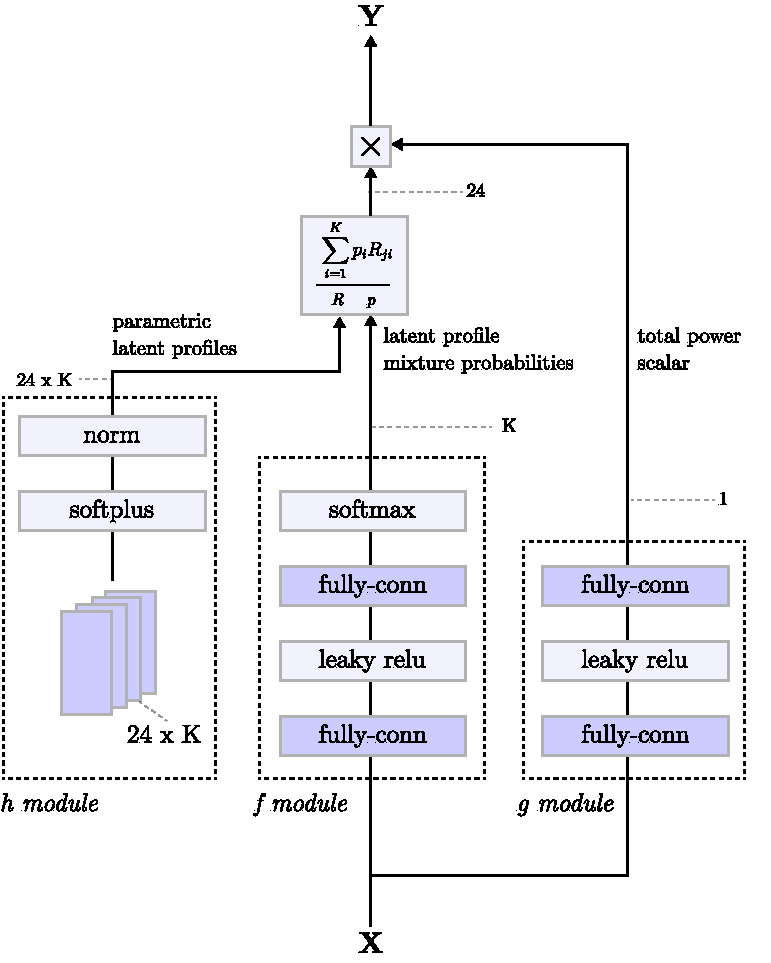
\includegraphics[width=0.8\textwidth]{nn-latent-architecture.pdf}
    \caption[Latent Neural Network Architecture]{Latent neural network architecture. Light blue rectangles denote NN layers without trainable parameters. While blue denotes layers with parameters learned by SGD. Notation borrowed from Fleurets book "Little book of deep learning"}
    \label{fig:nn-latent}
\end{figure}

The model is implemented in Python with use of Pytorch library \sidecite{paszke2019pytorchimperativestylehighperformance}.

\newpage


\section{Dataset splitting}
\label{sec:dataset-split}

To elaborate more on the way the datasets $\mathcal{T},\mathcal{S},\mathcal{V}$  are split. Since we are interested in modelling demand for location. We cannot just take all the \acrlong{APC}. Because of an issue, where one location has multiple \acrshort{ABM} for various \acrlong{TP} and also because the \acrshort{CS} has multiple \acrshort{CP}. And there might be a high correlation between the multiple \acrshort{CP} and our goal is for the model to be able to estimate demand for new locations. So the split is done based on location. Where features for each location can be only present in one of the sets.

% \begin{equation}
%     \begin{split}
%         \textit{train}:      \; \mathcal{T} & = ((x_i, y_i) \in X \times Y |\, i = 1,\dots, P) \\
%         \textit{test}:       \; \mathcal{S} & = ((x_i, y_i) \in X \times Y |\, i = 1,\dots, R) \\
%         \textit{validation}: \; \mathcal{V} & = ((x_i, y_i) \in X \times Y |\, i = 1,\dots, O)
%     \end{split}
% \end{equation}


\begin{itemize}
    \item[]
          \begin{equation}
              \label{eq:train}
              \textit{train}: \; \mathcal{T} = ((x_i, y_i) \in X \times Y |\, i = 1,\dots, P)
          \end{equation}

          This dataset is used for training the model with use of \acrlong{SGD} for empirical risk minimization.
          \vspace{3mm}
    \item[]  \begin{equation}
              \label{eq:test}
              \textit{test}:       \; \mathcal{S}  = ((x_i, y_i) \in X \times Y |\, i = 1,\dots, R)
          \end{equation}
          Is used for inspecting results of the model to see its performance on never seen data and tuning hyperparameters. And is used as an estimate of true model risk.
          \vspace{3mm}
    \item[]  \begin{equation}
              \label{eq:validation}
              \textit{validation}: \; \mathcal{V} = ((x_i, y_i) \in X \times Y |\, i = 1,\dots, O)
          \end{equation}
          This dataset is used to obtain the final model risk on model with already trained parameters and chosen hyperparameters.
\end{itemize}

\section{Training procedure}

\begin{itemize}
    \item SGD
    \item batches
    \item early stopping to avoid overfitting
    \item
\end{itemize}


\section{Other models for quantitative comparison}

The model is quantitatively compared with other models from the filed of machine learning. Results from the comparsion can motivate further research with the existing model or enable to quickly reject it.

One issue arrises from our custom loss, which is a mix with of two $L1$ losses. The ML models assume they want to minimize L1 loss. This might seem naive and not as a direct comparison hovewer more info will be provided in \ref{ch:results}.

The models for comparsion are the following:

\begin{itemize}
    \item \textbf{Average} - The most simple baseline. That is taking average over the whole datasets feature vectors and using that value as a prediction. Both the train and test datasets $\mathcal{T},\mathcal{S},$ are utilized for this "model". It does not take into account the input and utilizes one value for any further predictions.

          We provide the implementation.
          \begin{equation}
              \begin{split}
                   & f(z)^{\mathcal{D}}  = \frac{1}{|\mathcal{D}|} \sum_{(x,\_) \in \mathcal{D}} x \\
                   & f: \mathbb{R}^m \rightarrow \mathbb{R}^n                                      \\
                   & n,m \in \mathbb{N}, \mathcal{D} \in  (X \times Y)^p, p \in \mathbb{N}
              \end{split}
          \end{equation}


    \item \textbf{Linear regression} - Linear model

          Implementation is taken from Python library Scikit Learn \sidecite{scikit-learn}
          \begin{equation}
              \begin{split}
                   & f(z) = \alpha  + \beta z                                   \\
                   & f: \mathbb{R}^m \rightarrow \mathbb{R}^n                   \\
                   & \alpha \in \mathbb{R}^{n \times m}, \beta \in \mathbb{R}^n
              \end{split}
          \end{equation}
    \item \textbf{XGBoost} - A scalable end-to-end tree boosting system \sidecite{Chen_2016}
\end{itemize}

The perofrmacne of these models is compared with our model based on mean absolute error, mean square error on the following: \acrlong{APC}, \acrlong{TDPC} and \acrlong{NDPC}.